\documentclass[10pt,a4paper]{article}
\usepackage[utf8x]{inputenc}
\usepackage[spanish]{babel}
\usepackage{amsmath, amsbsy, amssymb, amsthm, amsfonts, latexsym}
\usepackage{graphicx}
\usepackage{multicol, multirow, rotating}
\usepackage{titling}
\usepackage{titlesec}
\usepackage{array}
\usepackage{bm}
\usepackage{afterpage}
\usepackage{float}
\usepackage{epstopdf}
\usepackage{longtable}
\usepackage{xcolor}
\usepackage{epigraph}
\setlength\epigraphwidth{1.5\textwidth}
\usepackage{subfigure}
\usepackage{anyfontsize}
\usepackage[left=2cm,right=2cm,top=2cm,bottom=2cm]{geometry}
\usepackage[colorlinks=true,linkcolor=blue,citecolor=blue,urlcolor=blue]{hyperref}
\usepackage{listings}
\renewcommand{\lstlistingname}{Programa}% Listing -> Programa
\renewcommand{\lstlistlistingname}{List of \lstlistingname s}
\lstset{tabsize=2,basicstyle=\small\ttfamily,breaklines=true,columns=fixed,extendedchars=true,prebreak = \raisebox{0ex}[0ex][0ex]{\ensuremath{\hookleftarrow}},tabsize=2,backgroundcolor=\color[HTML]{F0F0F0},identifierstyle=\ttfamily\color[HTML]{06287E},keywordstyle=\bfseries\color[HTML]{007020},commentstyle=\itshape\color[HTML]{60A0B0},stringstyle=\color[HTML]{4070A0}}
 %%%%%%%%%%%%%%%%%%%%%%%%%%%%%%%%%%%%%%%%%%%%%%%%%%%%%%%%%%%%%%%%%%%%%%%%%%%%%%%% 
%%% ~ Arduino Language - Arduino IDE Colors ~                                  %%%
%%%                                                                            %%%
%%% Kyle Rocha-Brownell | 10/2/2017 | No Licence                               %%%
%%% -------------------------------------------------------------------------- %%%
%%%                                                                            %%%
%%% Place this file in your working directory (next to the latex file you're   %%%
%%% working on).  To add it to your project, place:                            %%%
%%%     %%%%%%%%%%%%%%%%%%%%%%%%%%%%%%%%%%%%%%%%%%%%%%%%%%%%%%%%%%%%%%%%%%%%%%%%%%%%%%%% 
%%% ~ Arduino Language - Arduino IDE Colors ~                                  %%%
%%%                                                                            %%%
%%% Kyle Rocha-Brownell | 10/2/2017 | No Licence                               %%%
%%% -------------------------------------------------------------------------- %%%
%%%                                                                            %%%
%%% Place this file in your working directory (next to the latex file you're   %%%
%%% working on).  To add it to your project, place:                            %%%
%%%     %%%%%%%%%%%%%%%%%%%%%%%%%%%%%%%%%%%%%%%%%%%%%%%%%%%%%%%%%%%%%%%%%%%%%%%%%%%%%%%% 
%%% ~ Arduino Language - Arduino IDE Colors ~                                  %%%
%%%                                                                            %%%
%%% Kyle Rocha-Brownell | 10/2/2017 | No Licence                               %%%
%%% -------------------------------------------------------------------------- %%%
%%%                                                                            %%%
%%% Place this file in your working directory (next to the latex file you're   %%%
%%% working on).  To add it to your project, place:                            %%%
%%%    \input{arduinoLanguage.tex}                                             %%%
%%% somewhere before \begin{document} in your latex file.                      %%%
%%%                                                                            %%%
%%% In your document, place your arduino code between:                         %%%
%%%   \begin{lstlisting}[language=Arduino]                                     %%%
%%% and:                                                                       %%%
%%%   \end{lstlisting}                                                         %%%
%%%                                                                            %%%
%%% Or create your own style to add non-built-in functions and variables.      %%%
%%%                                                                            %%%
 %%%%%%%%%%%%%%%%%%%%%%%%%%%%%%%%%%%%%%%%%%%%%%%%%%%%%%%%%%%%%%%%%%%%%%%%%%%%%%%% 

\usepackage{color}
\usepackage{listings}    
\usepackage{courier}

%%% Define Custom IDE Colors %%%
\definecolor{arduinoGreen}    {rgb} {0.17, 0.43, 0.01}
\definecolor{arduinoGrey}     {rgb} {0.47, 0.47, 0.33}
\definecolor{arduinoOrange}   {rgb} {0.8 , 0.4 , 0   }
\definecolor{arduinoBlue}     {rgb} {0.01, 0.61, 0.98}
\definecolor{arduinoDarkBlue} {rgb} {0.0 , 0.2 , 0.5 }

%%% Define Arduino Language %%%
\lstdefinelanguage{Arduino}{
  language=C++, % begin with default C++ settings 
%
%
  %%% Keyword Color Group 1 %%%  (called KEYWORD3 by arduino)
  keywordstyle=\color{arduinoGreen},   
  deletekeywords={  % remove all arduino keywords that might be in c++
                break, case, override, final, continue, default, do, else, for, 
                if, return, goto, switch, throw, try, while, setup, loop, export, 
                not, or, and, xor, include, define, elif, else, error, if, ifdef, 
                ifndef, pragma, warning,
                HIGH, LOW, INPUT, INPUT_PULLUP, OUTPUT, DEC, BIN, HEX, OCT, PI, 
                HALF_PI, TWO_PI, LSBFIRST, MSBFIRST, CHANGE, FALLING, RISING, 
                DEFAULT, EXTERNAL, INTERNAL, INTERNAL1V1, INTERNAL2V56, LED_BUILTIN, 
                LED_BUILTIN_RX, LED_BUILTIN_TX, DIGITAL_MESSAGE, FIRMATA_STRING, 
                ANALOG_MESSAGE, REPORT_DIGITAL, REPORT_ANALOG, SET_PIN_MODE, 
                SYSTEM_RESET, SYSEX_START, auto, int8_t, int16_t, int32_t, int64_t, 
                uint8_t, uint16_t, uint32_t, uint64_t, char16_t, char32_t, operator, 
                enum, delete, bool, boolean, byte, char, const, false, float, double, 
                null, NULL, int, long, new, private, protected, public, short, 
                signed, static, volatile, String, void, true, unsigned, word, array, 
                sizeof, dynamic_cast, typedef, const_cast, struct, static_cast, union, 
                friend, extern, class, reinterpret_cast, register, explicit, inline, 
                _Bool, complex, _Complex, _Imaginary, atomic_bool, atomic_char, 
                atomic_schar, atomic_uchar, atomic_short, atomic_ushort, atomic_int, 
                atomic_uint, atomic_long, atomic_ulong, atomic_llong, atomic_ullong, 
                virtual, PROGMEM,
                Serial, Serial1, Serial2, Serial3, SerialUSB, Keyboard, Mouse,
                abs, acos, asin, atan, atan2, ceil, constrain, cos, degrees, exp, 
                floor, log, map, max, min, radians, random, randomSeed, round, sin, 
                sq, sqrt, tan, pow, bitRead, bitWrite, bitSet, bitClear, bit, 
                highByte, lowByte, analogReference, analogRead, 
                analogReadResolution, analogWrite, analogWriteResolution, 
                attachInterrupt, detachInterrupt, digitalPinToInterrupt, delay, 
                delayMicroseconds, digitalWrite, digitalRead, interrupts, millis, 
                micros, noInterrupts, noTone, pinMode, pulseIn, pulseInLong, shiftIn, 
                shiftOut, tone, yield, Stream, begin, end, peek, read, print, 
                println, available, availableForWrite, flush, setTimeout, find, 
                findUntil, parseInt, parseFloat, readBytes, readBytesUntil, readString, 
                readStringUntil, trim, toUpperCase, toLowerCase, charAt, compareTo, 
                concat, endsWith, startsWith, equals, equalsIgnoreCase, getBytes, 
                indexOf, lastIndexOf, length, replace, setCharAt, substring, 
                toCharArray, toInt, press, release, releaseAll, accept, click, move, 
                isPressed, isAlphaNumeric, isAlpha, isAscii, isWhitespace, isControl, 
                isDigit, isGraph, isLowerCase, isPrintable, isPunct, isSpace, 
                isUpperCase, isHexadecimalDigit, 
                }, 
  morekeywords={   % add arduino structures to group 1
                break, case, override, final, continue, default, do, else, for, 
                if, return, goto, switch, throw, try, while, setup, loop, export, 
                not, or, and, xor, include, define, elif, else, error, if, ifdef, 
                ifndef, pragma, warning,
                }, 
% 
%
  %%% Keyword Color Group 2 %%%  (called LITERAL1 by arduino)
  keywordstyle=[2]\color{arduinoBlue},   
  keywords=[2]{   % add variables and dataTypes as 2nd group  
                HIGH, LOW, INPUT, INPUT_PULLUP, OUTPUT, DEC, BIN, HEX, OCT, PI, 
                HALF_PI, TWO_PI, LSBFIRST, MSBFIRST, CHANGE, FALLING, RISING, 
                DEFAULT, EXTERNAL, INTERNAL, INTERNAL1V1, INTERNAL2V56, LED_BUILTIN, 
                LED_BUILTIN_RX, LED_BUILTIN_TX, DIGITAL_MESSAGE, FIRMATA_STRING, 
                ANALOG_MESSAGE, REPORT_DIGITAL, REPORT_ANALOG, SET_PIN_MODE, 
                SYSTEM_RESET, SYSEX_START, auto, int8_t, int16_t, int32_t, int64_t, 
                uint8_t, uint16_t, uint32_t, uint64_t, char16_t, char32_t, operator, 
                enum, delete, bool, boolean, byte, char, const, false, float, double, 
                null, NULL, int, long, new, private, protected, public, short, 
                signed, static, volatile, String, void, true, unsigned, word, array, 
                sizeof, dynamic_cast, typedef, const_cast, struct, static_cast, union, 
                friend, extern, class, reinterpret_cast, register, explicit, inline, 
                _Bool, complex, _Complex, _Imaginary, atomic_bool, atomic_char, 
                atomic_schar, atomic_uchar, atomic_short, atomic_ushort, atomic_int, 
                atomic_uint, atomic_long, atomic_ulong, atomic_llong, atomic_ullong, 
                virtual, PROGMEM,
                },  
% 
%
  %%% Keyword Color Group 3 %%%  (called KEYWORD1 by arduino)
  keywordstyle=[3]\bfseries\color{arduinoOrange},
  keywords=[3]{  % add built-in functions as a 3rd group
                Serial, Serial1, Serial2, Serial3, SerialUSB, Keyboard, Mouse, EEPROM,
                TimerOne},      
%
%
  %%% Keyword Color Group 4 %%%  (called KEYWORD2 by arduino)
  keywordstyle=[4]\color{arduinoOrange},
  keywords=[4]{  % add more built-in functions as a 4th group
                abs, acos, asin, atan, atan2, ceil, constrain, cos, degrees, exp, 
                floor, log, map, max, min, radians, random, randomSeed, round, sin, 
                sq, sqrt, tan, pow, bitRead, bitWrite, bitSet, bitClear, bit, 
                highByte, lowByte, analogReference, analogRead, 
                analogReadResolution, analogWrite, analogWriteResolution, 
                attachInterrupt, detachInterrupt, digitalPinToInterrupt, delay, 
                delayMicroseconds, digitalWrite, digitalRead, interrupts, millis, 
                micros, noInterrupts, noTone, pinMode, pulseIn, pulseInLong, shiftIn, 
                shiftOut, tone, yield, Stream, begin, end, peek, read, print, 
                println, available, availableForWrite, flush, setTimeout, find, 
                findUntil, parseInt, parseFloat, readBytes, readBytesUntil, readString, 
                readStringUntil, trim, toUpperCase, toLowerCase, charAt, compareTo, 
                concat, endsWith, startsWith, equals, equalsIgnoreCase, getBytes, 
                indexOf, lastIndexOf, length, replace, setCharAt, substring, 
                toCharArray, toInt, press, release, releaseAll, accept, click, move, 
                isPressed, isAlphaNumeric, isAlpha, isAscii, isWhitespace, isControl, 
                isDigit, isGraph, isLowerCase, isPrintable, isPunct, isSpace, 
                isUpperCase, isHexadecimalDigit, 
                },      
%
%
  %%% Set Other Colors %%%
  stringstyle=\color{arduinoDarkBlue},    
  commentstyle=\color{arduinoGrey},    
%          
%   
  %%%% Line Numbering %%%%
   numbers=left,                    
  numbersep=5pt,                   
  numberstyle=\color{arduinoGrey},    
  %stepnumber=2,                      % show every 2 line numbers
%
%
  %%%% Code Box Style %%%%
  breaklines=true,                    % wordwrapping
  tabsize=2,
  frame=shadowbox,
  rulesepcolor=\color{arduinoBlue},         
  basicstyle=\ttfamily  
}                                             %%%
%%% somewhere before \begin{document} in your latex file.                      %%%
%%%                                                                            %%%
%%% In your document, place your arduino code between:                         %%%
%%%   \begin{lstlisting}[language=Arduino]                                     %%%
%%% and:                                                                       %%%
%%%   \end{lstlisting}                                                         %%%
%%%                                                                            %%%
%%% Or create your own style to add non-built-in functions and variables.      %%%
%%%                                                                            %%%
 %%%%%%%%%%%%%%%%%%%%%%%%%%%%%%%%%%%%%%%%%%%%%%%%%%%%%%%%%%%%%%%%%%%%%%%%%%%%%%%% 

\usepackage{color}
\usepackage{listings}    
\usepackage{courier}

%%% Define Custom IDE Colors %%%
\definecolor{arduinoGreen}    {rgb} {0.17, 0.43, 0.01}
\definecolor{arduinoGrey}     {rgb} {0.47, 0.47, 0.33}
\definecolor{arduinoOrange}   {rgb} {0.8 , 0.4 , 0   }
\definecolor{arduinoBlue}     {rgb} {0.01, 0.61, 0.98}
\definecolor{arduinoDarkBlue} {rgb} {0.0 , 0.2 , 0.5 }

%%% Define Arduino Language %%%
\lstdefinelanguage{Arduino}{
  language=C++, % begin with default C++ settings 
%
%
  %%% Keyword Color Group 1 %%%  (called KEYWORD3 by arduino)
  keywordstyle=\color{arduinoGreen},   
  deletekeywords={  % remove all arduino keywords that might be in c++
                break, case, override, final, continue, default, do, else, for, 
                if, return, goto, switch, throw, try, while, setup, loop, export, 
                not, or, and, xor, include, define, elif, else, error, if, ifdef, 
                ifndef, pragma, warning,
                HIGH, LOW, INPUT, INPUT_PULLUP, OUTPUT, DEC, BIN, HEX, OCT, PI, 
                HALF_PI, TWO_PI, LSBFIRST, MSBFIRST, CHANGE, FALLING, RISING, 
                DEFAULT, EXTERNAL, INTERNAL, INTERNAL1V1, INTERNAL2V56, LED_BUILTIN, 
                LED_BUILTIN_RX, LED_BUILTIN_TX, DIGITAL_MESSAGE, FIRMATA_STRING, 
                ANALOG_MESSAGE, REPORT_DIGITAL, REPORT_ANALOG, SET_PIN_MODE, 
                SYSTEM_RESET, SYSEX_START, auto, int8_t, int16_t, int32_t, int64_t, 
                uint8_t, uint16_t, uint32_t, uint64_t, char16_t, char32_t, operator, 
                enum, delete, bool, boolean, byte, char, const, false, float, double, 
                null, NULL, int, long, new, private, protected, public, short, 
                signed, static, volatile, String, void, true, unsigned, word, array, 
                sizeof, dynamic_cast, typedef, const_cast, struct, static_cast, union, 
                friend, extern, class, reinterpret_cast, register, explicit, inline, 
                _Bool, complex, _Complex, _Imaginary, atomic_bool, atomic_char, 
                atomic_schar, atomic_uchar, atomic_short, atomic_ushort, atomic_int, 
                atomic_uint, atomic_long, atomic_ulong, atomic_llong, atomic_ullong, 
                virtual, PROGMEM,
                Serial, Serial1, Serial2, Serial3, SerialUSB, Keyboard, Mouse,
                abs, acos, asin, atan, atan2, ceil, constrain, cos, degrees, exp, 
                floor, log, map, max, min, radians, random, randomSeed, round, sin, 
                sq, sqrt, tan, pow, bitRead, bitWrite, bitSet, bitClear, bit, 
                highByte, lowByte, analogReference, analogRead, 
                analogReadResolution, analogWrite, analogWriteResolution, 
                attachInterrupt, detachInterrupt, digitalPinToInterrupt, delay, 
                delayMicroseconds, digitalWrite, digitalRead, interrupts, millis, 
                micros, noInterrupts, noTone, pinMode, pulseIn, pulseInLong, shiftIn, 
                shiftOut, tone, yield, Stream, begin, end, peek, read, print, 
                println, available, availableForWrite, flush, setTimeout, find, 
                findUntil, parseInt, parseFloat, readBytes, readBytesUntil, readString, 
                readStringUntil, trim, toUpperCase, toLowerCase, charAt, compareTo, 
                concat, endsWith, startsWith, equals, equalsIgnoreCase, getBytes, 
                indexOf, lastIndexOf, length, replace, setCharAt, substring, 
                toCharArray, toInt, press, release, releaseAll, accept, click, move, 
                isPressed, isAlphaNumeric, isAlpha, isAscii, isWhitespace, isControl, 
                isDigit, isGraph, isLowerCase, isPrintable, isPunct, isSpace, 
                isUpperCase, isHexadecimalDigit, 
                }, 
  morekeywords={   % add arduino structures to group 1
                break, case, override, final, continue, default, do, else, for, 
                if, return, goto, switch, throw, try, while, setup, loop, export, 
                not, or, and, xor, include, define, elif, else, error, if, ifdef, 
                ifndef, pragma, warning,
                }, 
% 
%
  %%% Keyword Color Group 2 %%%  (called LITERAL1 by arduino)
  keywordstyle=[2]\color{arduinoBlue},   
  keywords=[2]{   % add variables and dataTypes as 2nd group  
                HIGH, LOW, INPUT, INPUT_PULLUP, OUTPUT, DEC, BIN, HEX, OCT, PI, 
                HALF_PI, TWO_PI, LSBFIRST, MSBFIRST, CHANGE, FALLING, RISING, 
                DEFAULT, EXTERNAL, INTERNAL, INTERNAL1V1, INTERNAL2V56, LED_BUILTIN, 
                LED_BUILTIN_RX, LED_BUILTIN_TX, DIGITAL_MESSAGE, FIRMATA_STRING, 
                ANALOG_MESSAGE, REPORT_DIGITAL, REPORT_ANALOG, SET_PIN_MODE, 
                SYSTEM_RESET, SYSEX_START, auto, int8_t, int16_t, int32_t, int64_t, 
                uint8_t, uint16_t, uint32_t, uint64_t, char16_t, char32_t, operator, 
                enum, delete, bool, boolean, byte, char, const, false, float, double, 
                null, NULL, int, long, new, private, protected, public, short, 
                signed, static, volatile, String, void, true, unsigned, word, array, 
                sizeof, dynamic_cast, typedef, const_cast, struct, static_cast, union, 
                friend, extern, class, reinterpret_cast, register, explicit, inline, 
                _Bool, complex, _Complex, _Imaginary, atomic_bool, atomic_char, 
                atomic_schar, atomic_uchar, atomic_short, atomic_ushort, atomic_int, 
                atomic_uint, atomic_long, atomic_ulong, atomic_llong, atomic_ullong, 
                virtual, PROGMEM,
                },  
% 
%
  %%% Keyword Color Group 3 %%%  (called KEYWORD1 by arduino)
  keywordstyle=[3]\bfseries\color{arduinoOrange},
  keywords=[3]{  % add built-in functions as a 3rd group
                Serial, Serial1, Serial2, Serial3, SerialUSB, Keyboard, Mouse, EEPROM,
                TimerOne},      
%
%
  %%% Keyword Color Group 4 %%%  (called KEYWORD2 by arduino)
  keywordstyle=[4]\color{arduinoOrange},
  keywords=[4]{  % add more built-in functions as a 4th group
                abs, acos, asin, atan, atan2, ceil, constrain, cos, degrees, exp, 
                floor, log, map, max, min, radians, random, randomSeed, round, sin, 
                sq, sqrt, tan, pow, bitRead, bitWrite, bitSet, bitClear, bit, 
                highByte, lowByte, analogReference, analogRead, 
                analogReadResolution, analogWrite, analogWriteResolution, 
                attachInterrupt, detachInterrupt, digitalPinToInterrupt, delay, 
                delayMicroseconds, digitalWrite, digitalRead, interrupts, millis, 
                micros, noInterrupts, noTone, pinMode, pulseIn, pulseInLong, shiftIn, 
                shiftOut, tone, yield, Stream, begin, end, peek, read, print, 
                println, available, availableForWrite, flush, setTimeout, find, 
                findUntil, parseInt, parseFloat, readBytes, readBytesUntil, readString, 
                readStringUntil, trim, toUpperCase, toLowerCase, charAt, compareTo, 
                concat, endsWith, startsWith, equals, equalsIgnoreCase, getBytes, 
                indexOf, lastIndexOf, length, replace, setCharAt, substring, 
                toCharArray, toInt, press, release, releaseAll, accept, click, move, 
                isPressed, isAlphaNumeric, isAlpha, isAscii, isWhitespace, isControl, 
                isDigit, isGraph, isLowerCase, isPrintable, isPunct, isSpace, 
                isUpperCase, isHexadecimalDigit, 
                },      
%
%
  %%% Set Other Colors %%%
  stringstyle=\color{arduinoDarkBlue},    
  commentstyle=\color{arduinoGrey},    
%          
%   
  %%%% Line Numbering %%%%
   numbers=left,                    
  numbersep=5pt,                   
  numberstyle=\color{arduinoGrey},    
  %stepnumber=2,                      % show every 2 line numbers
%
%
  %%%% Code Box Style %%%%
  breaklines=true,                    % wordwrapping
  tabsize=2,
  frame=shadowbox,
  rulesepcolor=\color{arduinoBlue},         
  basicstyle=\ttfamily  
}                                             %%%
%%% somewhere before \begin{document} in your latex file.                      %%%
%%%                                                                            %%%
%%% In your document, place your arduino code between:                         %%%
%%%   \begin{lstlisting}[language=Arduino]                                     %%%
%%% and:                                                                       %%%
%%%   \end{lstlisting}                                                         %%%
%%%                                                                            %%%
%%% Or create your own style to add non-built-in functions and variables.      %%%
%%%                                                                            %%%
 %%%%%%%%%%%%%%%%%%%%%%%%%%%%%%%%%%%%%%%%%%%%%%%%%%%%%%%%%%%%%%%%%%%%%%%%%%%%%%%% 

\usepackage{color}
\usepackage{listings}    
\usepackage{courier}

%%% Define Custom IDE Colors %%%
\definecolor{arduinoGreen}    {rgb} {0.17, 0.43, 0.01}
\definecolor{arduinoGrey}     {rgb} {0.47, 0.47, 0.33}
\definecolor{arduinoOrange}   {rgb} {0.8 , 0.4 , 0   }
\definecolor{arduinoBlue}     {rgb} {0.01, 0.61, 0.98}
\definecolor{arduinoDarkBlue} {rgb} {0.0 , 0.2 , 0.5 }

%%% Define Arduino Language %%%
\lstdefinelanguage{Arduino}{
  language=C++, % begin with default C++ settings 
%
%
  %%% Keyword Color Group 1 %%%  (called KEYWORD3 by arduino)
  keywordstyle=\color{arduinoGreen},   
  deletekeywords={  % remove all arduino keywords that might be in c++
                break, case, override, final, continue, default, do, else, for, 
                if, return, goto, switch, throw, try, while, setup, loop, export, 
                not, or, and, xor, include, define, elif, else, error, if, ifdef, 
                ifndef, pragma, warning,
                HIGH, LOW, INPUT, INPUT_PULLUP, OUTPUT, DEC, BIN, HEX, OCT, PI, 
                HALF_PI, TWO_PI, LSBFIRST, MSBFIRST, CHANGE, FALLING, RISING, 
                DEFAULT, EXTERNAL, INTERNAL, INTERNAL1V1, INTERNAL2V56, LED_BUILTIN, 
                LED_BUILTIN_RX, LED_BUILTIN_TX, DIGITAL_MESSAGE, FIRMATA_STRING, 
                ANALOG_MESSAGE, REPORT_DIGITAL, REPORT_ANALOG, SET_PIN_MODE, 
                SYSTEM_RESET, SYSEX_START, auto, int8_t, int16_t, int32_t, int64_t, 
                uint8_t, uint16_t, uint32_t, uint64_t, char16_t, char32_t, operator, 
                enum, delete, bool, boolean, byte, char, const, false, float, double, 
                null, NULL, int, long, new, private, protected, public, short, 
                signed, static, volatile, String, void, true, unsigned, word, array, 
                sizeof, dynamic_cast, typedef, const_cast, struct, static_cast, union, 
                friend, extern, class, reinterpret_cast, register, explicit, inline, 
                _Bool, complex, _Complex, _Imaginary, atomic_bool, atomic_char, 
                atomic_schar, atomic_uchar, atomic_short, atomic_ushort, atomic_int, 
                atomic_uint, atomic_long, atomic_ulong, atomic_llong, atomic_ullong, 
                virtual, PROGMEM,
                Serial, Serial1, Serial2, Serial3, SerialUSB, Keyboard, Mouse,
                abs, acos, asin, atan, atan2, ceil, constrain, cos, degrees, exp, 
                floor, log, map, max, min, radians, random, randomSeed, round, sin, 
                sq, sqrt, tan, pow, bitRead, bitWrite, bitSet, bitClear, bit, 
                highByte, lowByte, analogReference, analogRead, 
                analogReadResolution, analogWrite, analogWriteResolution, 
                attachInterrupt, detachInterrupt, digitalPinToInterrupt, delay, 
                delayMicroseconds, digitalWrite, digitalRead, interrupts, millis, 
                micros, noInterrupts, noTone, pinMode, pulseIn, pulseInLong, shiftIn, 
                shiftOut, tone, yield, Stream, begin, end, peek, read, print, 
                println, available, availableForWrite, flush, setTimeout, find, 
                findUntil, parseInt, parseFloat, readBytes, readBytesUntil, readString, 
                readStringUntil, trim, toUpperCase, toLowerCase, charAt, compareTo, 
                concat, endsWith, startsWith, equals, equalsIgnoreCase, getBytes, 
                indexOf, lastIndexOf, length, replace, setCharAt, substring, 
                toCharArray, toInt, press, release, releaseAll, accept, click, move, 
                isPressed, isAlphaNumeric, isAlpha, isAscii, isWhitespace, isControl, 
                isDigit, isGraph, isLowerCase, isPrintable, isPunct, isSpace, 
                isUpperCase, isHexadecimalDigit, 
                }, 
  morekeywords={   % add arduino structures to group 1
                break, case, override, final, continue, default, do, else, for, 
                if, return, goto, switch, throw, try, while, setup, loop, export, 
                not, or, and, xor, include, define, elif, else, error, if, ifdef, 
                ifndef, pragma, warning,
                }, 
% 
%
  %%% Keyword Color Group 2 %%%  (called LITERAL1 by arduino)
  keywordstyle=[2]\color{arduinoBlue},   
  keywords=[2]{   % add variables and dataTypes as 2nd group  
                HIGH, LOW, INPUT, INPUT_PULLUP, OUTPUT, DEC, BIN, HEX, OCT, PI, 
                HALF_PI, TWO_PI, LSBFIRST, MSBFIRST, CHANGE, FALLING, RISING, 
                DEFAULT, EXTERNAL, INTERNAL, INTERNAL1V1, INTERNAL2V56, LED_BUILTIN, 
                LED_BUILTIN_RX, LED_BUILTIN_TX, DIGITAL_MESSAGE, FIRMATA_STRING, 
                ANALOG_MESSAGE, REPORT_DIGITAL, REPORT_ANALOG, SET_PIN_MODE, 
                SYSTEM_RESET, SYSEX_START, auto, int8_t, int16_t, int32_t, int64_t, 
                uint8_t, uint16_t, uint32_t, uint64_t, char16_t, char32_t, operator, 
                enum, delete, bool, boolean, byte, char, const, false, float, double, 
                null, NULL, int, long, new, private, protected, public, short, 
                signed, static, volatile, String, void, true, unsigned, word, array, 
                sizeof, dynamic_cast, typedef, const_cast, struct, static_cast, union, 
                friend, extern, class, reinterpret_cast, register, explicit, inline, 
                _Bool, complex, _Complex, _Imaginary, atomic_bool, atomic_char, 
                atomic_schar, atomic_uchar, atomic_short, atomic_ushort, atomic_int, 
                atomic_uint, atomic_long, atomic_ulong, atomic_llong, atomic_ullong, 
                virtual, PROGMEM,
                },  
% 
%
  %%% Keyword Color Group 3 %%%  (called KEYWORD1 by arduino)
  keywordstyle=[3]\bfseries\color{arduinoOrange},
  keywords=[3]{  % add built-in functions as a 3rd group
                Serial, Serial1, Serial2, Serial3, SerialUSB, Keyboard, Mouse, EEPROM,
                TimerOne},      
%
%
  %%% Keyword Color Group 4 %%%  (called KEYWORD2 by arduino)
  keywordstyle=[4]\color{arduinoOrange},
  keywords=[4]{  % add more built-in functions as a 4th group
                abs, acos, asin, atan, atan2, ceil, constrain, cos, degrees, exp, 
                floor, log, map, max, min, radians, random, randomSeed, round, sin, 
                sq, sqrt, tan, pow, bitRead, bitWrite, bitSet, bitClear, bit, 
                highByte, lowByte, analogReference, analogRead, 
                analogReadResolution, analogWrite, analogWriteResolution, 
                attachInterrupt, detachInterrupt, digitalPinToInterrupt, delay, 
                delayMicroseconds, digitalWrite, digitalRead, interrupts, millis, 
                micros, noInterrupts, noTone, pinMode, pulseIn, pulseInLong, shiftIn, 
                shiftOut, tone, yield, Stream, begin, end, peek, read, print, 
                println, available, availableForWrite, flush, setTimeout, find, 
                findUntil, parseInt, parseFloat, readBytes, readBytesUntil, readString, 
                readStringUntil, trim, toUpperCase, toLowerCase, charAt, compareTo, 
                concat, endsWith, startsWith, equals, equalsIgnoreCase, getBytes, 
                indexOf, lastIndexOf, length, replace, setCharAt, substring, 
                toCharArray, toInt, press, release, releaseAll, accept, click, move, 
                isPressed, isAlphaNumeric, isAlpha, isAscii, isWhitespace, isControl, 
                isDigit, isGraph, isLowerCase, isPrintable, isPunct, isSpace, 
                isUpperCase, isHexadecimalDigit, 
                },      
%
%
  %%% Set Other Colors %%%
  stringstyle=\color{arduinoDarkBlue},    
  commentstyle=\color{arduinoGrey},    
%          
%   
  %%%% Line Numbering %%%%
   numbers=left,                    
  numbersep=5pt,                   
  numberstyle=\color{arduinoGrey},    
  %stepnumber=2,                      % show every 2 line numbers
%
%
  %%%% Code Box Style %%%%
  breaklines=true,                    % wordwrapping
  tabsize=2,
  frame=shadowbox,
  rulesepcolor=\color{arduinoBlue},         
  basicstyle=\ttfamily  
}

\begin{document}
\author{Velasco Angel}
\title{UNIVERSIDAD TÉCNICA DEL NORTE \\
FICA-CIERCOM\\
PERCEPTRÓN SIMPLE EN ARDUINO}
\maketitle
\section{Introducción}
En el mundo existe cada vez una mayor necesidad de la tecnología en la vida cotidiana de las personas, esta se usa desde en un cuarto de estudio hasta en una cocina.\\
Una de las ramas de la ingeniería donde más se ha profundizado en investigación y experimentación es la inteligencia artificial (AI), esta se ha venido desarrollando a través de los años y se ha llegado a obtener resultados bastante acertados, hoy en día una máquina es capaz de reconocer rostros en una foto, o incluso saber qué hay en una imagen con un extenso algoritmo de machine learning detrás. \\

Con este propósito nacen las famosas redes neuronales, cuya función es tener la posibilidad de reconocer y clasificar objetos con el uso de ciertos aspectos determinantes de dicho objeto.

\section{Marco Teórico}
\subsection{Sistema Neuronal Artificial}
1888 Ramón y Cajal demuestra que el sistema nervioso está compuesto por
una red de células individuales, las neuronas, ampliamente interconectadas
entre sí \cite{Larranaga}.\\
La información fluye desde las dendritas hacia el axón atravesando el soma. El cerebro se modela durante el desarrollo de un ser vivo. Algunas cualidades del ser humano no son innatas, sino adquiridas por la influencia de la
información que del medio externo se proporciona a sus sensores \cite{Larranaga}.

\subsubsection{Modelo estándar de neurona artificial}
Se va a introducir el denominado modelo estándar de neurona artificial según los
principios descritos en Rumelhart y McClelland (1986) y McClelland y Rumelhart (1986). Siguiendo dichos principios, la i-ésima neurona artificial estándard
consiste en:
\begin{itemize}
\item[$*$] Un conjunto de entradas $x_j$ y unos pesos sinápticos $w_{ij}$, con $j=1,...,n$.
\item[$*$] Una regla de propagación $h_i$ definida a partir del conjunto de entradas y los pesos sinápticos.
\item[$*$] una función de activación la cual representa simultáneamente la salida de
la neurona y su estado de activación.
La Figura~\ref{red} muestra el modelo de neurona artificial estándar descrito previamente.
\end{itemize}

\begin{figure}[H]
\centering
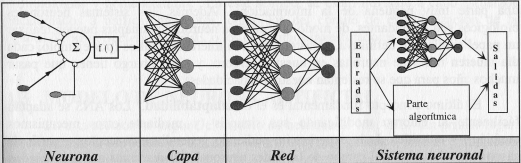
\includegraphics[scale=1]{sist_neuronal}
\caption{Sistema neuronal global de proceso de una red neuronal {\scriptsize \textbf{Fuente: }sh.ehu.es}}
\label{sistema}
\end{figure}

	

%\begin{table}[H]
%  	\centering
%  	\caption{Matriz de confusión}
%	\begin{tabular}{c  >{\centering\arraybackslash}m{2cm}|>{\centering\arraybackslash}m{3cm}| >{\centering\arraybackslash}m{3cm}|}
%		\cline{3-4} 
% 		&		& \multicolumn{2}{c|}{\textbf{Predicción}} \\
%		\cline{3-4}  
% 		&		& \textbf{Positivos} & \textbf{Negativos}\\
%		\hline 
%		\multicolumn{1}{|c|}{\multirow{2}{*}{\rotatebox{90}{\textbf{Observación}}}} 		& \textbf{Positivos} & Verdaderos Positivos (VP) & Falsos Negativos (FN)\\ 			[0.7cm]
%		\cline{2-4} 
%		\multicolumn{1}{|c|}{} 	& \textbf{Negativos} & Falsos Positivos (FP) & 				Verdaderos Negativos (VN) \\ [0.7cm]
%		\hline 
%	\end{tabular}%
%	\label{tab:confusion}%
%\end{table}


\subsection{Perceptrón Simple}
El perceptrón simple fue introducido por Rosenblatt (1962) y es un modelo unidireccional compuesto por dos capas de neuronas, una de entrada y otra de salida. La operación en un perceptrón simple que consta de $n$ neuronas de entrada y $m$ neuronas de salida, se puede expresar como:
\begin{equation}
y_i=f \left(\sum_{j=1}^{m} w_{ij} x_j - \theta_i \right)
\end{equation}
con $i=1,...,m$.\\

Las neuronas de entrada son discretas y la función de activación de las neuronas de
la capa de salida es de tipo escalón, Como se observa en la Figura~\ref{perc}.\\

\begin{figure}[H]
\centering
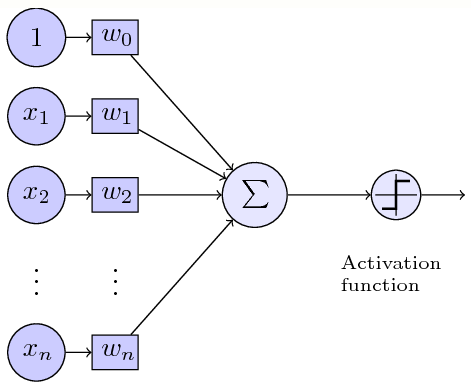
\includegraphics[scale=0.7]{perceptron}
\caption{Diagrama de Perceptrón {\scriptsize \textbf{Fuente: }https://tex.stackexchange.com/questions/104334/tikz-diagram-of-a-perceptron}}
\label{perc}
\end{figure}

Veamos con un ejemplo sencillo, que contiene dos neuronas de entrada, que el perceptrón simple tan solo puede discriminar entre dos clases linealmente separables, es decir, clases cuyas regiones de decisión pueden ser separadas mediante una única condición lineal o hiperplano \cite{BIBING2017}.\\
Si denotamos por $x1$ y $x2$ a las dos neuronas de entrada, la operación efectuada por el perceptrón simple consiste en:

\begin{equation}
y = \left\{\begin{matrix}
1, si & w_1x_1+w_2x_2 > \theta\\ 
0, si & w_1x_1+w_2x_2\leqslant \theta
\end{matrix}\right.
\end{equation}

Si consideramos $x_1$ y $x_2$ situadas sobre los ejes de abcisas y ordenadas respectivamente, la condición

\begin{equation}
w_1x_1+w_2x_2 -\theta=0
\end{equation}

es equivalente a:

\begin{equation}
x_2=-\frac{w_1}{w_2} x_1 + \frac{\theta}{w_2}
\end{equation}

y representa una recta (Figura~\ref{grafica}) que define la región de decisión determinada por el perceptrón simple. Es por ello que dicho perceptrón simple representa un discriminador lineal, al implementar una condición lineal que separa dos regiones en el espacio que representan dos clases diferentes de patrones \cite{BIBING2017}.\\

Por tanto, el perceptrón simple presenta grandes limitaciones, ya que tan sólo es capaz de representar funciones linealmente separables.

\begin{figure}[H]
\centering
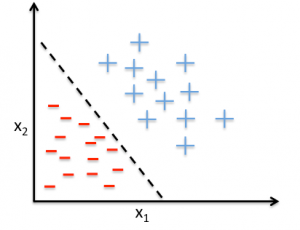
\includegraphics[scale=0.7]{per_grafica}
\caption{Región de decisión de Perceptrón Simple {\scriptsize \textbf{Fuente: }https://geeks.ms/mrcabellom/2017/08/04/perceptron-binario-en-machine-learning/}}
\label{grafica}
\end{figure}

\subsection{Red Neuronal Artificial}
Se puede definir una red neuronal artificial como un grafo dirigido (Figura~\ref{red}), con las siguientes propiedades:
\begin{enumerate}
\item A cada nodo (neurona) $i$ se le asocia una variable de estado $X_i$.
\item A cada conexión $(i, j)$ entre los nodos (neuronas) $i$ y $j$ se le asocia un peso $w_(ij) \in \mathbb{R}$.
\item A cada nodo (neurona) $i$ se le asocia un umbral $\theta_i \in \mathbb{R}$.
\item Para cada nodo $i$ se define una función $f_i(x_i,...,x_n,w_{i1},...,w_{in},\theta_i)$ que depende de los pesos de sus conexiones, del umbral y de los estados de los nodos $j$ que estén conectados con el nodo $i$. El valor de esta función proporciona el nuevo estado del nodo.

\end{enumerate}

Por lo que respecta a la terminología habitual en redes neuronales artificiales,
tal y como se ha comentado previamente los nodos del grafo representan a las
neuronas y las conexiones a las sinapsis. Se denominan neuronas de entrada a
aquellas neuronas sin sinapsis entrantes. A las neuronas sin sinapsis salientes
se las denomina neuronas de salida, y finalmente a aquellas neuronas que no
son ni de entrada ni de salida se les denomina neuronas ocultas. Una red es
unidireccional cuando no presenta bucles cerrados o conexiones, mientras que una
red se dice recurrente o realimentada cuando el flujo de información puede tener
un bucle de atras hacia adelante, es decir, una realimentación. En la relación con
la manera en la que las neuronas de una red actualizan sus estados, podemos
distinguir entre dinámica síncrona (en la cual todas las neuronas pertenecientes
a una misma capa se actualizan a la vez, comenzando en la capa de entrada y
continuando hasta la de salida) y dinámica asíncrona (en la cual cada neurona
actualiza su estado sin atender a cuando lo hacen las demás neuronas). Si bien
el tipo de dinámica presente en los sistemas neuronales biológicos es asíncrono,
lo habitual en las redes neuronales artificiales es que la dinámica sea síncrona \cite{Larranaga}.

\begin{figure}[H]
\centering
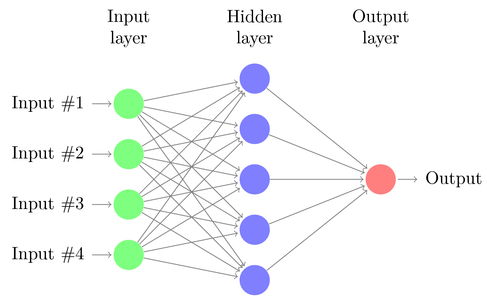
\includegraphics[scale=0.7]{red}
\caption{Partes de una red neuronal {\scriptsize \textbf{Fuente: }http://www.texample.net/tikz/examples/neural-network/}}
\label{red}
\end{figure}





\section{Desarrollo}
\subsection{Perceptrón en Arduino}
Para comenzar a programar nuestro perceptrón debemos tener en cuenta los siguientes aspectos:
\begin{itemize}
\item La base de datos a utilizar será la que tomamos en nuestro proyecto final (\href{https://github.com/JampyVi98/Sistemas-Embebidos/tree/master/Examen_Perceptron}{Ver Base de Datos}).
\item Esta base de datos cuenta con 300 datos (150 de etiqueta 1 y 150 de etiqueta 2) por 4 entradas y una salida de dos estados, ya que al tratarse de un preceptrón simple debemos trabajar con una ecuación lineal.
\item Al tener 4 entradas tendremos también 4 pesos sinápticos y a su vez un umbral ($\theta$ o $w_0$ como se aprecia en la Figura~\ref{perc}).
\item Por último hay que tomar en cuenta que las etiquetas que se tomaron en cuenta son $1$ y $2$, esto quiere decir que:

\begin{equation}
y = \left\{\begin{matrix}
1, si & w_1x_1+w_2x_2 > \theta\\ 
2, si & w_1x_1+w_2x_2\leqslant \theta
\end{matrix}\right.
\end{equation}

\end{itemize}

Con estas premicias, pasamos a la programación de nuestra neurona como se muestra en el Programa~\ref{cod:codigo}.

\lstinputlisting[language=Arduino, caption={Código Perceptrón Simple en Arduino}\label{cod:codigo}]{Examen_Perceptron/Examen_Perceptron.ino}


El código se lo puede encontrar en el siguiente \href{https://github.com/JampyVi98/Sistemas-Embebidos/tree/master/Examen_Perceptron}{enlace de GitHub}.

\section{Resultados}
Los resultados obtenidos en la práctica son muy satisfactorios, ya que se ha obtenido un rendimiento que supera por completo los clasificadores probados anteriormente.\\

Primeramente, en la Figura~\ref{ok} se presentan los datos donde la etiqueta predecida concuerda con la etiqueta original de los datos que se encuentran en la base. Asimismo, en la Figura~\ref{f} se presentan los datos donde la etiqueta predecida y la original no concuerdan entre sí.

\begin{figure}[htbp]
\centering

\begin{subfigure}{7a}
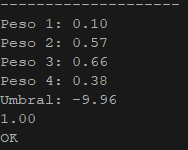
\includegraphics[scale=1]{ok}
\caption{Dato acertado}
\label{ok}
\end{subfigure}

\begin{subfigure}{7b}
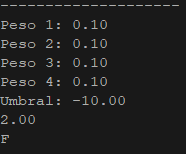
\includegraphics[scale=1]{fail}
\caption{Dato erróneo}
\label{f}
\end{subfigure}

\caption{Presentación de datos}
\label{datos}
\end{figure}

Por último, en la Figura~\ref{res} se presentan los resultados finales con el número de aciertos, número de errores y rendimiento expresado porcentualmente.


\begin{figure}[H]
\centering
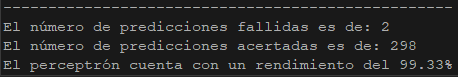
\includegraphics[scale=1]{resultado}
\caption{Resultados de rendimiento}
\label{res}
\end{figure}

\section{Conclusiones y Recomendaciones}


\subsection*{Conclusiones}
\begin{itemize}
\item Un perceptrón es la unidad mínima de una red neuronal, con una sola neurona hemos sido capaces de crear un clasificador bastante eficiente, con una red neuronal compuesta por algunos perceptrones tiene muchos más cálculos detrás pero viene a ser un dispositivo muy robusto y útil.
\item El factor de aprendizaje determina qué tan rápido nuestro algoritmo puede ser para aprender nuevos valores de peso para obtener una respuesta clara, si es muy bajo el prorama necesitará mayor número de iteraciones para llegar a un peso eficiente.
\item El perceptrón de una capa, a pesar de su simplicidad ha logrado superar con creces al clasificador K-nn y el clasificador Bayesiano.
\end{itemize}

\subsection*{Recomendaciones}
\begin{itemize}
\renewcommand{\labelitemi}{$*$}
\item Utilizar vectores o matrices en agrupaciones de datos para facilitar la programación.
\item Realizar un esquema gráfico y matemático sobre cómo trabajará el algoritmo.
\item Programar primeramente el algoritmo en un software más sencillo como lo es Excel, esto nos dará una idea más clara de los pasos que debemos seguir.
\end{itemize}




\bibliographystyle{ieeetran}%estilo referencia
\bibliography{Referencias}%archivo.bib
\end{document}